%%%%%%%%%%%%%%%%%%%%%%%%%%%%%%%%%%%%%%%%%
% Large Colored Title Article
% LaTeX Template
% Version 1.1 (25/11/12)
%
% This template has been downloaded from:
% http://www.LaTeXTemplates.com
%
% Original author:
% Frits Wenneker (http://www.howtotex.com)
%
% License:
% CC BY-NC-SA 3.0 (http://creativecommons.org/licenses/by-nc-sa/3.0/)
%
%%%%%%%%%%%%%%%%%%%%%%%%%%%%%%%%%%%%%%%%%

%----------------------------------------------------------------------------------------
%	PACKAGES AND OTHER DOCUMENT CONFIGURATIONS
%----------------------------------------------------------------------------------------

\documentclass[DIV=calc, paper=a4, fontsize=11pt, twocolumn]{scrartcl}	 % A4 paper and 11pt font size

\usepackage{graphicx}
\usepackage{hyperref}
\usepackage{lipsum} % Used for inserting dummy 'Lorem ipsum' text into the template
\usepackage[english]{babel} % English language/hyphenation
\usepackage[protrusion=true,expansion=true]{microtype} % Better typography
\usepackage{amsmath,amsfonts,amsthm} % Math packages
\usepackage[svgnames]{xcolor} % Enabling colors by their 'svgnames'
\usepackage[hang, small,labelfont=bf,up,textfont=it,up]{caption} % Custom captions under/above floats in tables or figures
\usepackage{booktabs} % Horizontal rules in tables
\usepackage{fix-cm}	 % Custom font sizes - used for the initial letter in the document

\usepackage{sectsty} % Enables custom section titles
\allsectionsfont{\usefont{OT1}{phv}{b}{n}} % Change the font of all section commands

\usepackage{fancyhdr} % Needed to define custom headers/footers
\pagestyle{fancy} % Enables the custom headers/footers
\usepackage{lastpage} % Used to determine the number of pages in the document (for "Page X of Total")

% Headers - all currently empty
\lhead{}
\chead{}
\rhead{}

% Footers
\lfoot{}
\cfoot{}
\rfoot{\footnotesize Page \thepage\ of \pageref{LastPage}} % "Page 1 of 2"

\renewcommand{\headrulewidth}{0.0pt} % No header rule
\renewcommand{\footrulewidth}{0.4pt} % Thin footer rule

\usepackage{lettrine} % Package to accentuate the first letter of the text
\newcommand{\initial}[1]{ % Defines the command and style for the first letter
\lettrine[lines=3,lhang=0.3,nindent=0em]{
\color{DarkGoldenrod}
{\textsf{#1}}}{}}

%----------------------------------------------------------------------------------------
%	TITLE SECTION
%----------------------------------------------------------------------------------------

\usepackage{titling} % Allows custom title configuration

\newcommand{\HorRule}{\color{DarkGoldenrod} \rule{\linewidth}{1pt}} % Defines the gold horizontal rule around the title

\pretitle{\vspace{-30pt} \begin{flushleft} \HorRule \fontsize{50}{50} \usefont{OT1}{phv}{b}{n} \color{DarkRed} \selectfont} % Horizontal rule before the title

\title{\Huge Literature Search Made Easy: Mining Online Archives for Research Topic Trends} % Your article title

\posttitle{\par\end{flushleft}\vskip 0.5em} % Whitespace under the title

\preauthor{\begin{flushleft}\large \lineskip 0.5em \usefont{OT1}{phv}{b}{sl} \color{DarkRed}} % Author font configuration

\author{Bo Wang, Min Liu } % Your name

\postauthor{\footnotesize \usefont{OT1}{phv}{m}{sl} \color{Black} % Configuration for the institution name
Stanford University % Your institution

\par\end{flushleft}\HorRule} % Horizontal rule after the title

\date{} % Add a date here if you would like one to appear underneath the title block

%----------------------------------------------------------------------------------------

\begin{document}

\maketitle % Print the title

\thispagestyle{fancy} % Enabling the custom headers/footers for the first page 

%----------------------------------------------------------------------------------------
%	ABSTRACT
%----------------------------------------------------------------------------------------

% The first character should be within \initial{}
\initial{M}\textbf{any of us have been faced with this situation: we found a certain field of research intriguing, went to an online archive to search for related papers, and the results were just less than satisfactory: they are too unstructured to obtain a big picture, such as how this field evolves over time, what sub-fields it is composed of, which papers are most influential, and who are the most active researchers. Instead of relying on human instinct for such insights, our project provides an alternative: using machine learning algorithms to peruse thru online archives, generate information of interest, and present them in a human friendly way. We scrape thousands of papers' title, abstract and author information from arXiv, use hierarchical latent Dirichlet allocation (hLDA), dynamic topic model (DTM) and supervised latent Dirichlet allocation (sLDA) to analyze the data. Interpretation and discussion of the results are also offered.}

%----------------------------------------------------------------------------------------
%	ARTICLE CONTENTS
%----------------------------------------------------------------------------------------

\section*{Data Collection}

We crawl the data from the online archive website arXiv. In fields like mathematics and physics, almost all scientific papers are self-archived on the arXiv. Despite not peer reviewed, arXiv has its submissions reviewed (or even recategorized if off-topic) by moderators that are experts in their fields of research. In addition, submission dates on arXiv more accurately reflect when the research was done, since usually papers are posted on arXiv months before they are finally published on a peer reviewed journal or conference. Based on these facts, we believe arXiv is a better collection of research works than any journal or conference alone.

The titles, authors, abstracts and citation of papers are scraped from API of \url{http://export.arxiv.org/api/} using Python and stored in separate files according to the publish year. We used only papers from the "condensed matter physics" section so far, since this is the field that we are familiar with and would be able to interpret the results better. But the methods demonstrated in this report can be applied to the analysis any field.

\section*{Methods}

\subsection*{Latent Dirichlet Allocation (LDA)}
Latent Dirichlet Allocation (LDA) \cite{2} is a topic modeling algorithm which assumes that each document is a mixture of various topics, whose prior distribution takes a Dirichlet distribution. In LDA, the number of topics is given a priori.

\subsection*{Hierarchical Latent Dirichlet Allocation (hLDA)}
For the purpose of hierarchical clustering of topics, we used hierarchical latent Dirichlet allocation(hLDA) \cite{1}, which is a variation of latent Dirichlet allocation(LDA) \cite{2} that finds a hierarchy of topics based on their similarities. Details of the algorithms will be added to the report later. Finding the hierarchy allows us to get a grasp of a field from a top-down point of view. 

\subsection*{Dynamic Topic Model (DTM)}
Dynamic topic models (DTM) \cite{3} are generative models that can be used to analyze the evolution of topics of a collection of documents over time. It is an extension of LDA which can handle sequential documents.\newline
In LDA, both the order the words appear in a document and the order the documents appear in the corpus are oblivious to the model. Whereas words are still assumed to be exchangeable, in a dynamic topic model the order of the documents plays a fundamental role. More precisely, the documents are grouped by time slice (e.g.: years) and it is assumed that the documents of each group come from a set of topics that evolved from the set of the previous slice.
\subsection*{Supervised Latent Dirichlet Allocation (sLDA)}
Supervised latent Dirichlet allocation (sLDA) is a statistical model of labelled documents, which can be used to predict response values for new documents. In this project, we plan to use sLDA to model the number of citations of each paper, and predict the importance of new papers based on the fitted model.
\section*{Experiments}

We used abstracts of the first 6000 submissions to the condensed matter section as our corpus. A term matrix generator (TMG) \cite{3} with stop words filter is used to generate a dictionary containing all terms that appeared in at least 5 documents and a term matrix whose (i, j)-th element n denotes that the j-th word in our dictionary occurred n times in the i-th document. The resulting matrix had 19327 terms and was fed thru an off the shelf C-package "hlda-c" \cite{1} implementing hLDA.\\
A depth 4 tree generated by "hlda-c" looks like:\newline
			\begin{figure}[!ht]
				\centerline{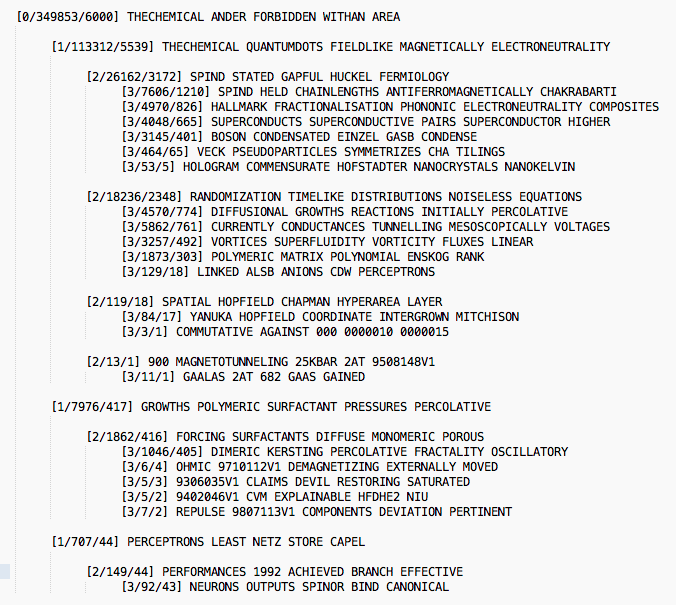
\includegraphics[scale = 0.35]{tree10000.png}}
				\caption{Unsupervised Hierarchical Classification of First 10000 Submissions to Condensed Matter Physics Section}
			\end{figure}
\newline
Despite being completely unsupervised, the result is actually surprisingly good. The three numbers in square brackets before each line are tree level, number of terms and number of documents in this branch. The top node (0th - level ) contains the function words. In the next level, the documents are classified into three branches: first class containing 5539 documents, second class containing 417 documents and the third class containing 44 documents. Eventhough the dataset seem to very skewed, with the largest class containing 100 times more documents than the smallest class, the classification captures sub fields in condensed matter physics very nicely: the first class is still very large, so its keywords are still pretty much function words, but if we go a level down to level 2, we can see the first branch contains mostly theoretical studies on correlated systems such as superconductors, antiferromagnet, quantum Hall and Bose Eistein condensation; the second branch contains experimental papers on material growth and transport measurements; Second class on level 1 is topics on studies in the intersection of condensed matter physics and chemistry, namely material synthesis; third branch on level 1 contains topics on computational physics -- using computational methods to calculate physical and chemical properties of materials. The hierarchical clustering not only gives us a very good idea what the sub fields are, but also ranked them according to their popularity, which agrees well with our knowledge of the field.      

\section*{Milestone: Progress So Far}
So far we have done the following tasks.
\begin{enumerate}
\item Crawled paper titles and abstracts from arXiv
\item Indexed data into term-frequency matrix
\item Transformed data to the LDA input format
\item Clustered with LDA and hLDA
\item Obtained and analyzed initial results
\end{enumerate}

\section*{Milestone: Next Step}
For the next step, we have following plans.
\begin{enumerate}
\item Cluster data with DTM and analyze the evolution of research topics
\item Train and compare the results of sLDA
\item Do experiments with data from different sub domains (e.g. high energy physics, astro physics) and macro domains (e.g. computer science, mathematics)
\end{enumerate}

\section*{Acknowlegement}
We would like to thank the TAs for their guidance and advice for this project. We also want to thank Prof. Andrew Ng for such for introducing us to the exciting field of machine learning.  
%----------------------------------------------------------------------------------------
%	REFERENCE LIST
%----------------------------------------------------------------------------------------

\begin{thebibliography}{99}

\bibitem[1] {1}
  Blei, D., Griffiths, T. and Jordan M.
  \emph{The Nested Chinese Restaurant Process and Bayesian Nonparametric Inference of Topic Hierarchies}.
  Journal of the ACM, Vol. 57, No. 2, Article 7,
 Jan 2010.
 
\bibitem[2] {2}
  Blei, D., Ng, A. and Jordan M.
  \emph{Latent Dirichlet Allocation}.
  The Journal of Machine Learning Research,
 Volume 3, 993 - 1022
 Mar 2003
 
<<<<<<< HEAD
\bibitem[3] {3}
  D. Zeimpekis and E. Gallopoulos
  \emph{TMG: A MATLAB-based term-document Matrix Constructor for Text Collections}.
  Technical Report, Computer Engineering and Information Department, University of Patras
  Dec 2003
  http://scgroup20.ceid.upatras.gr:8000/tmg/

=======
 \bibitem[3] {3}
  Blei, D. and Lafferty, J.
  \emph{Dynamic Topic Models}.
  Proceedings of the 23rd International Conference of Machine Learning ,
 Pittsburgh, PA,
 2006
 
 \bibitem[4] {4}
  Blei, D. and McAuliffe, J.
  \emph{Supervised Topic Models}.
 
>>>>>>> bafd9488b0620cbc23e36139c2e176c506b35283
\end{thebibliography}
%----------------------------------------------------------------------------------------

\end{document}